\section{Refactoring}

\begin{frame}{Pattern di Refactoring}
    Tra i numerossissimi pattern di refactoring utilizzati nello sviluppo dell'applicazione abbiamo selezionato solo i più rilevanti (sia dal punto di vista della frequenza di utilizzo sia dal punto di vista degli effetti positivi che la loro applicazione ha sul codice). \\\bigskip
    Tali pattern sono:
    \begin{itemize}
        \item Extract Class
        \item Extract Method
        \item Replace Temp with Query
        \item Extract Constant
    \end{itemize}
    Mostreremo nel dettaglio solo alcuni di essi.
    
\end{frame}

\begin{frame}{Pattern di Refactoring}
    \framesubtitle{Pattern Extract Class}
    
    \begin{figure}
        \centering
        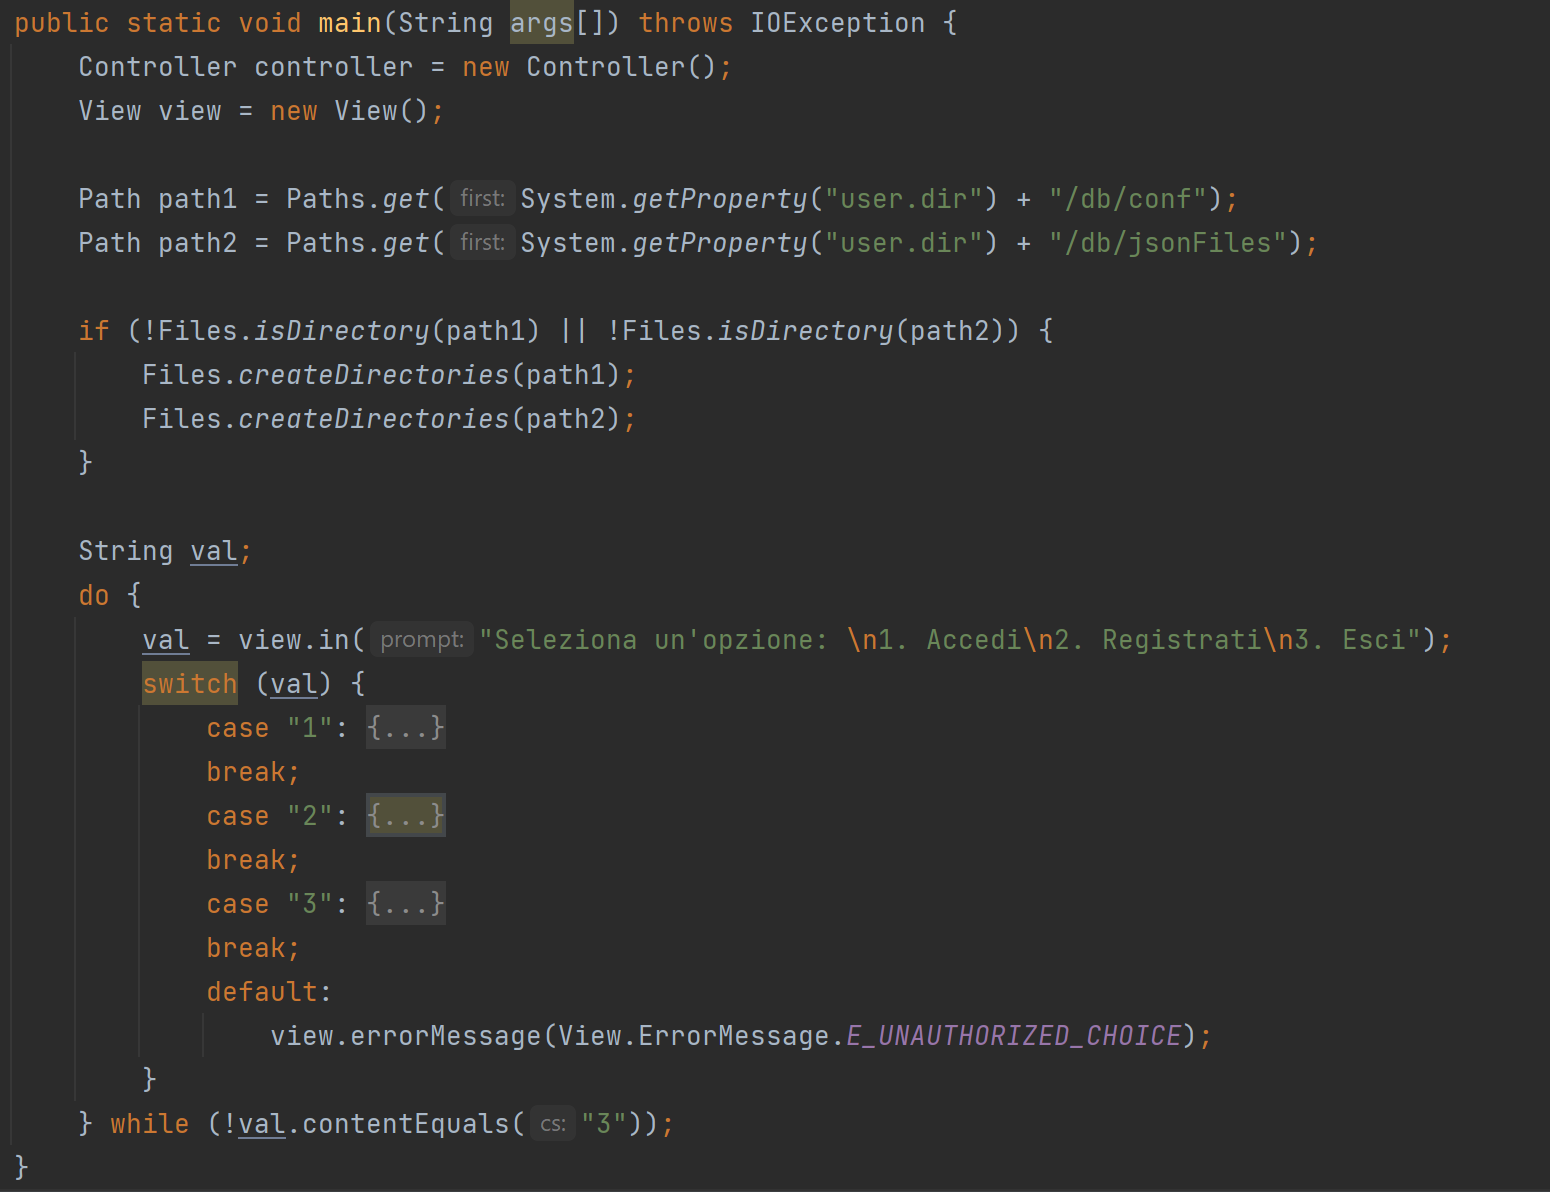
\includegraphics[width=.65\textwidth]{refactoring/extractclass1.png}
    \end{figure}    

    \note{
        Il nostro metodo \texttt{main} nella versione 5 aveva la struttura presentata nell'immagine.\\
        Chiaramente esso violava svariati principi di buona programmazione (primo tra tutti SRP, in quanto si occupava sia di creare le directories che di permettere all'utente di effettuare la scelta di un'azione da eseguire).\\\bigskip
        Abbiamo suddiviso le responsabilità creando una classe \texttt{LocalPath} che si occupa della creazione delle directories in cui creare e recuperare i file \texttt{json} di configurazione e delle gerarchie.
    }
\end{frame}

\begin{frame}{Pattern di Refactoring}
    \framesubtitle{Pattern Extract Class}
    
    \begin{figure}
        \centering
        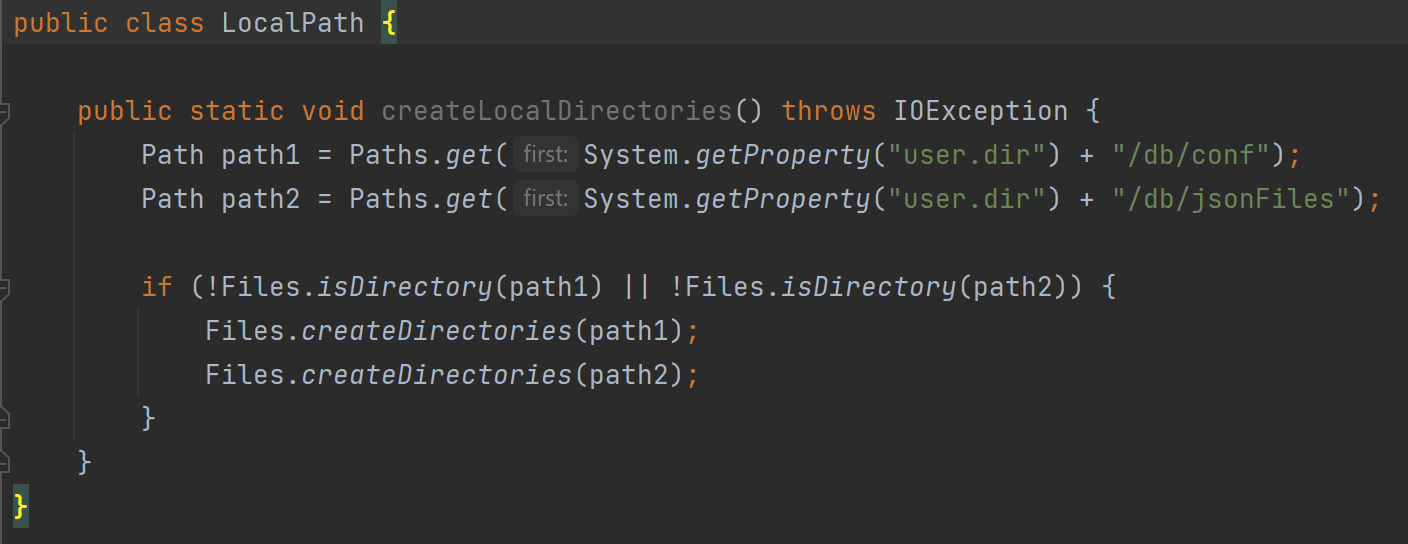
\includegraphics[width=.7\textwidth]{refactoring/extractclass2.png}
    \end{figure}    

    \note{
        Nella classe \texttt{LocalPath} abbiamo creato un metodo statico contenente il codice necessario per creare le directories. 
        In questo modo il metodo potrà essere chiamato direttamente nel \texttt{main} invocandolo dalla classe.
    }
\end{frame}

\begin{frame}{Pattern di Refactoring}
    \framesubtitle{Pattern Extract Method e Replace Temp with Query}
    
    \begin{figure}
        \centering
        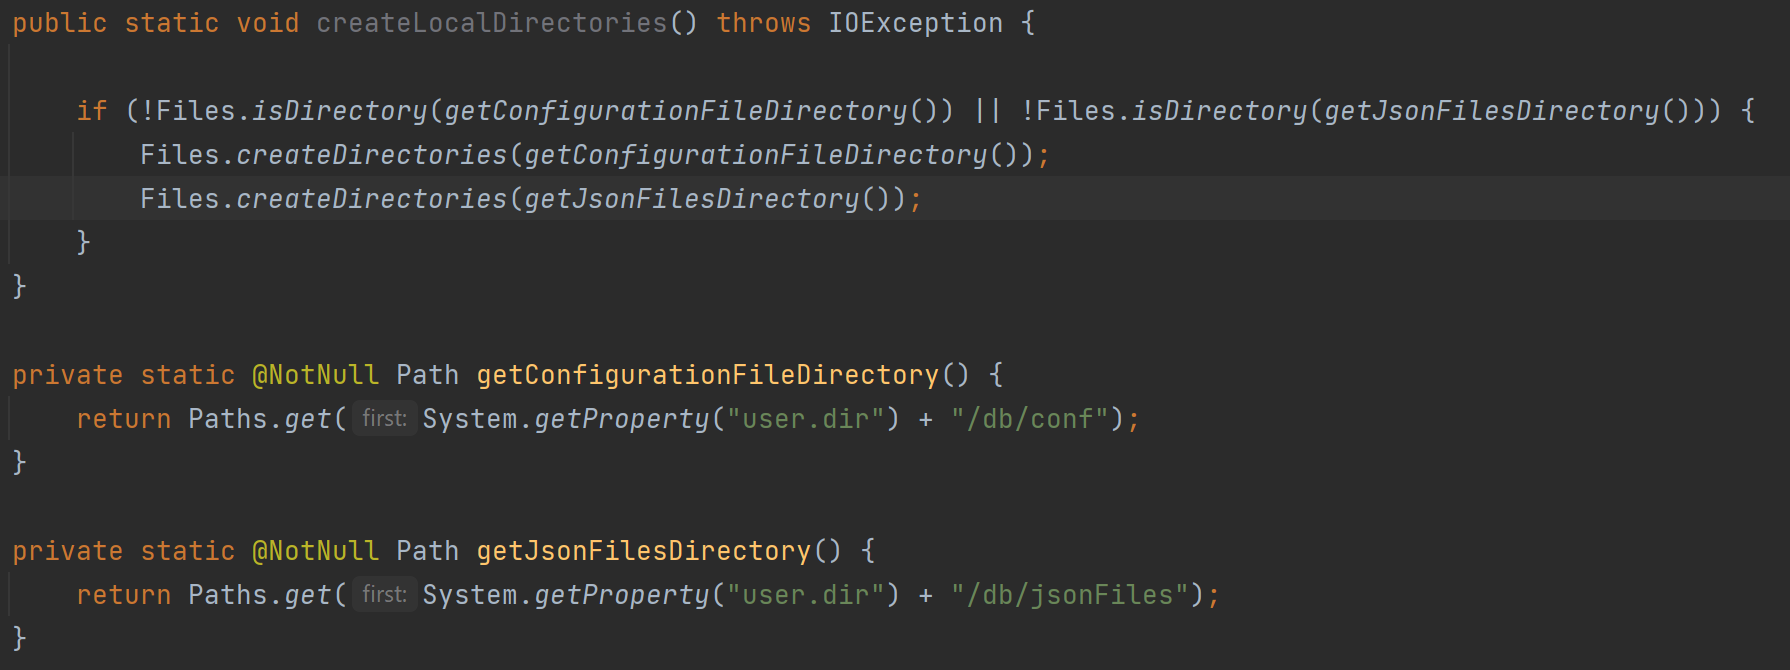
\includegraphics[width=.7\textwidth]{refactoring/extractclass3.png}
    \end{figure}    

    \note{
       Abbiamo poi estratto i metodi per individuare il \textit{path} delle directories, sempre all'interno della classe \texttt{LocalPath}.\\
       Si tratta di un'applicazione del pattern di refactoring ``Extract Method''. \\\bigskip
       Inoltre, anziché creare delle variabili temporanee per salvare localmente i \textit{path} trovati, abbiamo applicato la tecnica di refactoring ``Replace temp with Query''.\\
       Ciò è stato possibile in virtù del fatto che i metodi per ricavare i \textit{path} sono idempotenti, pertanto la loro invocazione ripetuta non ha effetti collaterali sul sistema.
    }
\end{frame}

\begin{frame}{Pattern di Refactoring}
    \framesubtitle{Pattern Extract Constant}
    
    \begin{figure}
        \centering
        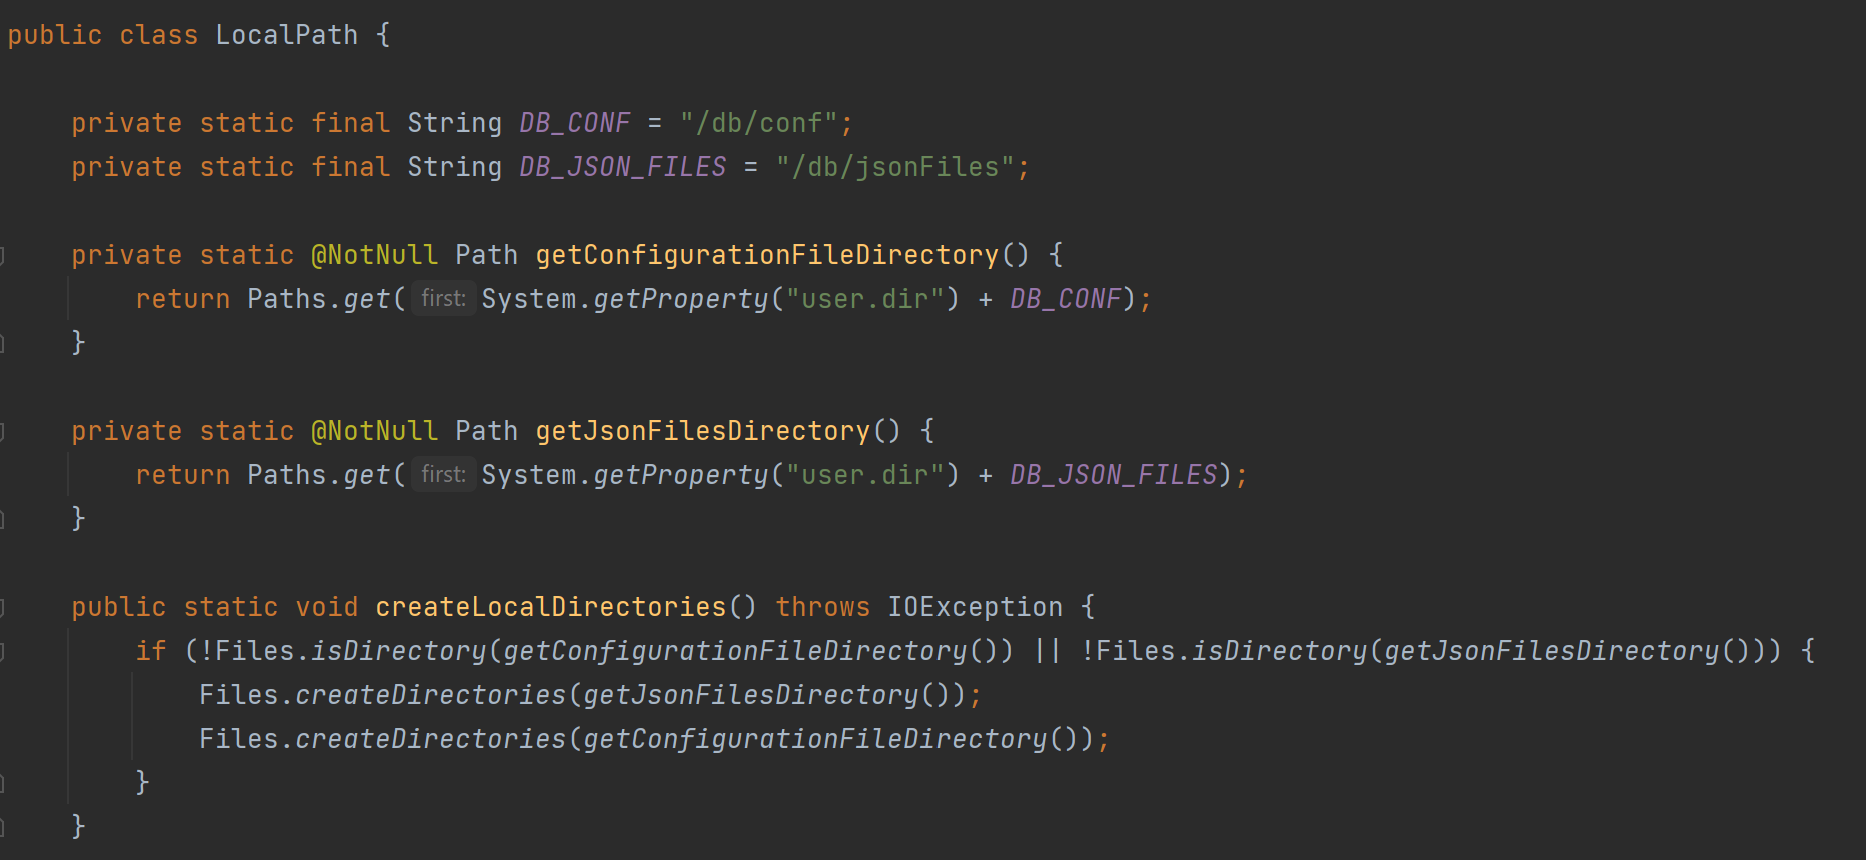
\includegraphics[width=.7\textwidth]{refactoring/extractclass4.png}
    \end{figure}    

    \note{
       Abbiamo poi rapidamente estratto le costanti \texttt{final} per indicare i \textit{path} in modo da poter in futuro consentire modifiche ai \textit{path} stessi accedendo a un solo punto dell'applicazione. \\
       In questo caso è stato applicato il pattern di refactoring ``Extract constant''.\\\bigskip
       La classe LocalPath è così ultimata (a meno di modifiche introdotte solo successivamente per la gestione della creazione delle liste di \textit{path} delle directories dei file \texttt{json} da caricare). 
    }
\end{frame}

\begin{frame}{Pattern di Refactoring}
    
    \begin{figure}
        \centering
        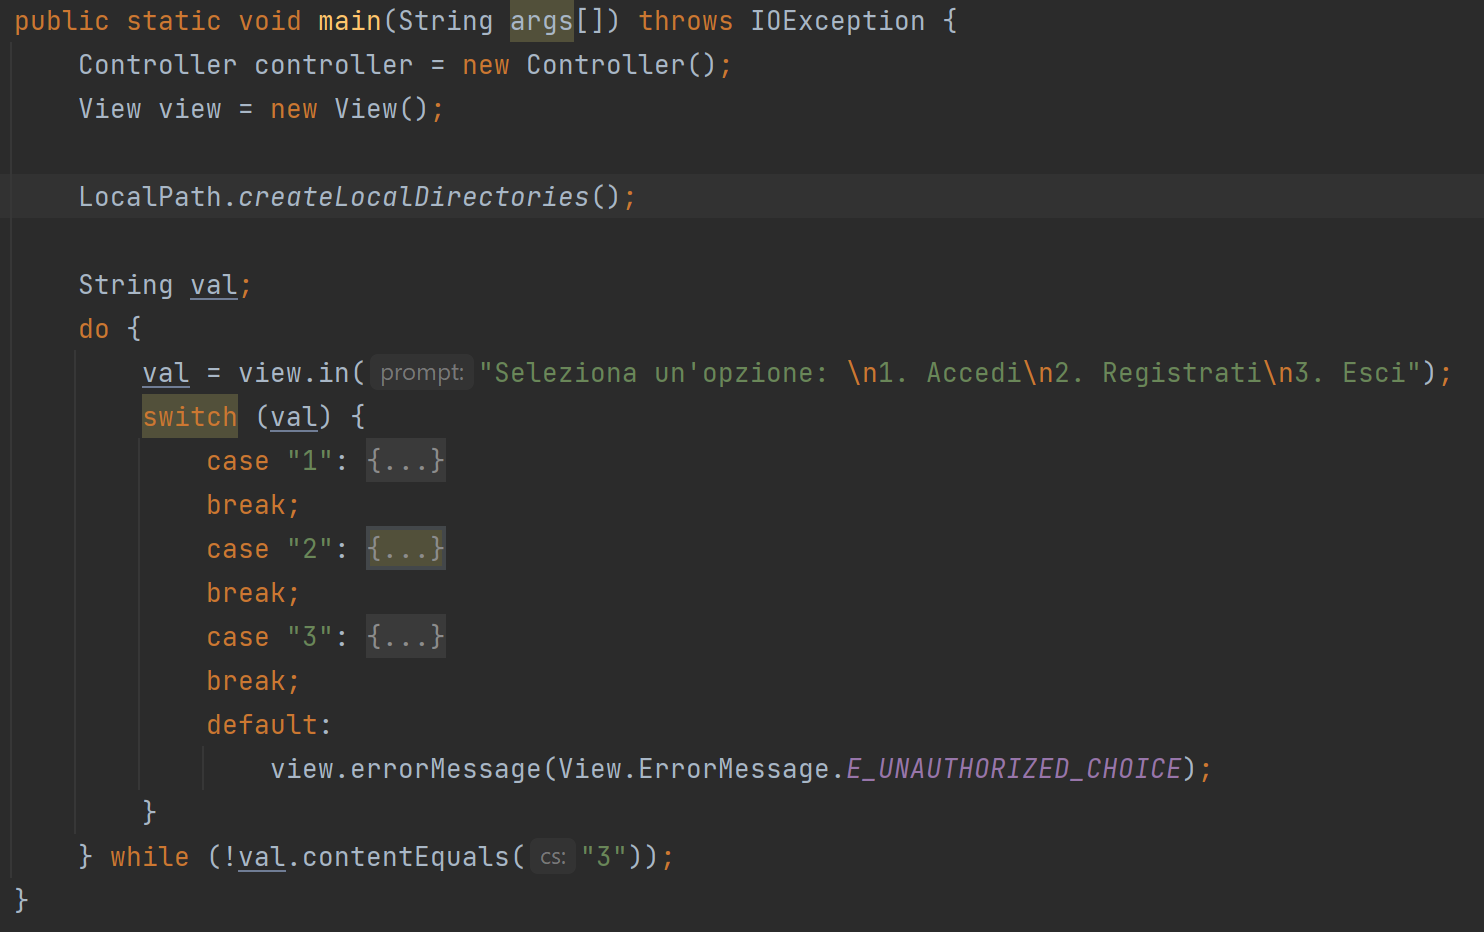
\includegraphics[width=.7\textwidth]{refactoring/extractclass5.png}
    \end{figure}    

    \note{
       Infine abbiamo richiamato il metodo statico della classe appena creata nel metodo \texttt{main}.
    }
\end{frame}